\documentclass{article}

\usepackage[utf8]{inputenc}
\usepackage[francais]{babel}
\usepackage[T1]{fontenc}
\usepackage{lmodern}
\usepackage{graphicx}
\usepackage{caption}
\usepackage{subcaption}
\usepackage{epstopdf}
\usepackage{array}
\usepackage{amsmath}
\usepackage{amssymb}
\usepackage{amsfonts}
\usepackage{amsopn}
\usepackage[usenames,dvipsnames]{color}
\usepackage[left=3cm,right=3cm,top=2.5cm,bottom=2.5cm]{geometry}

\usepackage{listings}
\definecolor{gray}{rgb}{0.4,0.4,0.4}
\definecolor{dkgreen}{rgb}{0.25,0.7,0.35}
\definecolor{dkred}{rgb}{0.7,0,0} 
\lstset{language=matlab,numbers=left,numberstyle=\tiny\color{gray},basicstyle=\rm\footnotesize,keywordstyle=\bfseries\color{dkred},frame=single,commentstyle=\color{gray}=small, stringstyle=\color{dkgreen}}

% Numbers and units
\usepackage[squaren, Gray]{SIunits}
\usepackage{sistyle}
\usepackage[autolanguage]{numprint}
%\usepackage{numprint}
\newcommand\si[2]{\numprint[#2]{#1}}
\newcommand\np[1]{\numprint{#1}}

% Matlab import
\usepackage{xparse}% for using parameters at the end block
\NewDocumentEnvironment{mylist}{m}{%
  \begin{#1}%
  % other code
}{%
  \end{#1}%
}

\NewDocumentEnvironment{mytable}{mm}
{\begin{table}[!ht]\centering}
{\caption{#2 Valeurs obtenues par le code du listing~\ref{lst:#1}.}\label{tab:#1}\end{table}}

\newcommand{\matlabplot}[2]
{\begin{figure}[!ht]\centering
\includegraphics[width=\textwidth]{img/#1.png}
\caption{#2 Graphique obtenu par le code du listing~\ref{lst:#1}.}\label{fig:#1}\end{figure}}


\newcommand{\matlabcode}[2]
{\lstinputlisting[caption={Contenu du fichier \lstinline{#1.m}
  contenant l'implémentation de la fonction \lstinline{#1}.
#2},label={lst:#1}]
{matlab/#1.m}
}

\DeclareMathOperator{\var}{Var}

\title{LFSAB1105 : APP 2013-2014 \\ Probabilités et statistiques}
\author{
\begin{tabular}{llll}
\textsc{Legat} & Benoît & 4896-11-00\\
\textsc{Peschke} & Lena & 5826-11-00\\
\textsc{Sanchez Falcon} & Alexandre & 2912-11-00\\
\textsc{Sedda} & Mélanie & 2246-11-00\\
\end{tabular}}
\date{\today}

\begin{document}
\maketitle

\begin{center}
\line(1,0){250}
\end{center}

Tous les codes Matlab auquel nous ferons référence se trouvent dans l'Annexe A de rapport.
\section{Question 1}
\subsection{Méthode des moments}
\subsection{Méthode graphique}
Soit l'échantillon aléatoire $X_1$,...,$X_n$ obtenu avec la loi de densité suivante (définie pour $x \geq 0$, avec $k$ et $c > 0$) :
$$ f(x) = \frac{k}{c}\left(\frac{x}{c}\right)^{k-1}\exp\left[-\left(\frac{x}{c}\right)^{k}\right] $$ 
On aimerait trouver un estimateur $\hat{\theta} = (\hat{k},\hat{c})$ pour $\theta = (k,c)$ en utilisant la régression linéaire.
Pour cela, notons que
$$ \ln(-\ln(1-F(x))) = k\ln(x)-k\ln(c) $$
Il suffit alors de choisir des points $x$ et d'estimer $F(x)$ grâce aux données empiriques $X_1$,...,$X_n$. La régression linéaire nous donnera des estimateurs $\hat{k}$ et $-\hat{k}\ln(\hat{c})$ dont nous pouvons facilement extraire $\hat{\theta}$. Pour simplifier les choses, on peut réindicer $X_1$,...,$X_n$ en $X_1'$,...,$X_n'$, de telle sorte que $X_1'<X_2'<$...$<X_n'$ (on suppose les $X_i$ obtenus différents). On évalue alors très simplement $F$ en chaque $X_i'$ : 
$$ \hat{F}(X_i') = i/n $$
On peut alors utiliser les $n-1$ premières valeurs de $X'$ pour effectuer la régression linéaire (le soucis avec la dernière c'est que $\hat{F}(X_n') = 1$ et donc $\ln(1-F)$ n'est pas défini).
\subsection{Méthode du maximum de vraisemblance}
\paragraph{Démonstration}
\noindent On a l'équation de maximum de vraisemblance : \\
\begin{equation}
\mbox{L}\left(\mbox{k },\alpha \right) = \left( \mbox{k} \alpha^{k} \right)^{n} \left( \prod\limits_{i=1}^{n} \mbox{x}^{\mbox{k}-1}_{i} \right) \mbox{exp}\left( -\alpha^{k} \sum\limits_{i=1}^n \mbox{x}^{k}_{i}\right)
\end{equation}
où $\alpha$ = $\dfrac{1}{c}$ . \\
Ensuite, nous travaillerons avec $\hat{\mbox{l}}$ = log$\left( \mbox{L} \right)$ tel que : 
\begin{equation}
\hat{\mbox{l}}(\mbox{k},\alpha) = \mbox{nlog}(\mbox{k}) + \mbox{nk log}(\alpha) + (\mbox{k}-1) \sum\limits_{i=1}^{n}\mbox{log}(\mbox{x}_{i}) - \alpha^{k} \sum\limits_{i=1}^{n} \mbox{x}^{k}_{i}
\end{equation}
avec $\hat{\mbox{l}}$ décomposer au maximum sous la forme d'une somme. Ainsi, nous pourrons obtenir aisément les dérivées de $\hat{\mbox{l}}$. \\
Calculons donc :
\begin{align}
\dfrac{\partial\hat{\mbox{l}}(\mbox{k},\alpha)}{\partial \alpha} &= \mbox{nk} \dfrac{1}{\alpha} - \sum\limits_{i=1}^{n} \mbox{x}^{k}_{i} \left( \mbox{k} \alpha^{\mbox{k}-1} \right) = 0 \label{eq:la} \\ \label{eq:lk}
\dfrac{\partial\hat{\mbox{l}}(\mbox{k},\alpha)}{\partial \mbox{k}} &= \dfrac{\mbox{n}}{\mbox{k}} + \mbox{n}\mbox{log}(\alpha) + \sum\limits_{i=1}^{n} \mbox{log}(\mbox{x}^{k}_{i}) - \sum\limits_{i=1}^{n} \dfrac{(\partial \alpha \mbox{x}_{i})^{\mbox{k}}}{\partial \mbox{k}} = 0
\end{align}
Développons l'équation \ref{eq:la} en multipliant l'équation par $\alpha$ :
\begin{equation}
\mbox{n} = \sum\limits_{i=1}^{n} \mbox{x }^{k}_{i} \alpha^{\mbox{k}} 
\end{equation}
Il vient donc directement par la définition de $\alpha$ que :
\begin{equation}
\mbox{c} = \left(\sum\limits_{i=1}^{n} \mbox{x }^{k}_{i}\dfrac{1}{\mbox{n}}\right)^{\dfrac{1}{\mbox{k}}} \label{c}
\end{equation}
Développons à présent l'équation \ref{eq:lk}. \\ 
Nous utiliserons par ailleurs la propriété de dérivation suivante :
\begin{equation}
\dfrac{\partial \mbox{a}^{\mbox{x}}}{\partial \mbox{x}} = \mbox{log}(\mbox{a})~\mbox{a}^{\mbox{x}}
\end{equation}
Ainsi, nous avons après avoir développé la dernière dérivée partielle de l'équation \ref{eq:lk} :
\begin{equation}
 \dfrac{\mbox{n}}{\mbox{k}} + \mbox{n}\mbox{log}(\alpha) + \sum\limits_{i=1}^{n} \mbox{log}(\mbox{x}^{k}_{i}) -  \sum\limits_{i=1}^{n}  \left[ \left[ \mbox{log}(\mbox{x}_{i}) + \mbox{log}(\alpha) \right] \alpha^{\mbox{k}} \mbox{x}^{k}_{i} \right] = 0
\end{equation}
Nous pouvons encore simplifier l'expression ci-dessus en utilisant l'équation \ref{c} :
\begin{equation}
\sum\limits_{i=1}^{n}  \left[ \left[ \mbox{log}(\mbox{x}_{i}) + \mbox{log}(\alpha) \right] \alpha^{\mbox{k}} \mbox{x}^{k}_{i} \right] = \mbox{n} \dfrac{\sum\limits_{i=1}^{n} \mbox{x}^{k}_{i} \mbox{~log}(\mbox{x}_{i})}{\sum\limits_{i=1}^{n} \mbox{x}^{k}_{i}} + \mbox{n}\mbox{log}(\alpha)
\end{equation}
Nous arrivons donc à l'équation suivante en annulant les termes en log($\alpha$):
\begin{equation}
\dfrac{\mbox{n}}{\mbox{k}} = \mbox{n} \dfrac{\sum\limits_{i=1}^{n} \mbox{x}^{k}_{i} \mbox{~log}(\mbox{x}_{i})}{\sum\limits_{i=1}^{n} \mbox{x}^{k}_{i}} - \sum\limits_{i=1}^{n} \mbox{~log}(\mbox{x}_{i})
\end{equation}
et nous obtenons le résultat souhaité :
\begin{equation}
\dfrac{1}{\mbox{k}} = \dfrac{\sum\limits_{i=1}^{n} \mbox{x}^{k}_{i} \mbox{~log}(\mbox{x}_{i})}{\sum\limits_{i=1}^{n} \mbox{x}^{k}_{i}} - \dfrac{\sum\limits_{i=1}^{n} \mbox{~log}(\mbox{x}_{i})}{\mbox{n}}
\end{equation}

%b)
\paragraph{Echantillon, points candidats et fonction de vraisemblance}
La fonction \texttt{wblmle} nous permet de trouver un estimateur par la méthode du maximum de vraisemblance pour un échantillon aléatoire simple qui suit une loi de densité
$ f(x)= \frac{k}{c} \left(\frac{x}{c}\right)^{k-1} \exp \left[ -\left(\frac{x}{c}\right)^{k}\right] \mathbb{I}\{x \geq 0\}$ avec $k>0$ et $c>0$.
%b)
La première étape consiste à générer un échantillon $X_1,...,X_n$. Nous utilisons pour ce faire la fonction \texttt{wblrnd} avec un paramètre  $\theta$ au choix. Pour la suite de l'explication, posons $\theta = (k,c) = (3.7, 4.2)$. Nous construisons ensuite une grille de points candidats autour des valeurs de $k$ et $c$. La grille contient $101$ paires de point variant entre $(0.7k, 0.7c)$ et $(1.3k, 1.3c)$. Pour chaque paire de points, nous calculons le logarithme de la fonction de vraisemblance depuis la fonction \texttt{wblloglike}~:
$$LL(\theta=(k,c)) = \sum_{i=1}^{n}{\ln(f(x_i;\theta=(k,c)))} = n\ln(k) - kn\ln(c) + \sum_{i=1}^{n}{\left[(k-1)\ln(x_i) - \left(\frac{x_i}{c}\right)^{k}\right]}$$

\paragraph{Estimateurs et maximum de vraisemblance} Une fois les 101 points candidats évalués, nous cherchons le maximum parmi eux pour déterminer le $k$ et $c$ qui lui correspondent et qui deviennent $\hat{k}_{MLE}$ et $\hat{c}_{MLE}$, nos estimateurs de choix. C'est ce qui correspond à l'étape analytique $\frac{\partial LL(\theta)}{\partial \theta} = 0$.

%c)
\paragraph{Un exemple} En exécutant \texttt{wblmle(1000, 4.2, 3.7)} (où $n = 1000$ le nombre de $X_i$, $c = 4.2$, $k = 3.7$), nous obtenons, par exemple, $\hat{k}_{MLE} = 3.7000$ et $\hat{c}_{MLE} = 4.2504$.
L'erreur quadratique totale pour ces valeurs est $ERT_{MLE} = (\hat{k}_{MLE} - k)^2 + (\hat{c}_{MLE} - c)^2 = 0.0025$.

%d)
\paragraph{500 \'echantillons} La routine \texttt{MLE\_replicate} nous permet ensuite d'effectuer un certain nombre de réplications d'échantillons aléatoires simples et de calculer leurs $\hat{k}_{MLE}$, $\hat{c}_{MLE}$ et $ERT_{MLE}$ respectifs. Pour chacune des trois séries, nous calculons la moyenne et la variance. Les valeurs obtenues sont reprises dans la table~\ref{table:mle}.

\begin{table}[!ht]
\centering
\begin{tabular}{|l|l|l|}
\hline
				& Moyenne 	& Variance\\
\hline
$\hat{k}_{MLE}$ & 3.7006 	& 0.0086\\
$\hat{c}_{MLE}$ & 4.2003 	& 0.0014\\
$ERT_{MLE}$			& 0.0100	& 0.0001\\
\hline
\end{tabular}
\caption{Valeurs obtenues avec la méthode du maximum de vraisemblance pour 500 échantillons.}
\label{table:mle}
\end{table}

%e)
Pour chaque série, nous avons produit un box-plot et un histogramme. Les graphes relatifs à $\hat{k}_{MLE}$ se retrouvent à la figure~\ref{fig:kmle}, ceux de $\hat{c}_{MLE}$ à la figure~\ref{fig:cmle} et ceux de $ERT_{MLE}$ à la figure~\ref{fig:ertmle}.

\begin{figure}[!ht]
        \centering
        \begin{subfigure}[b]{0.5\textwidth}
                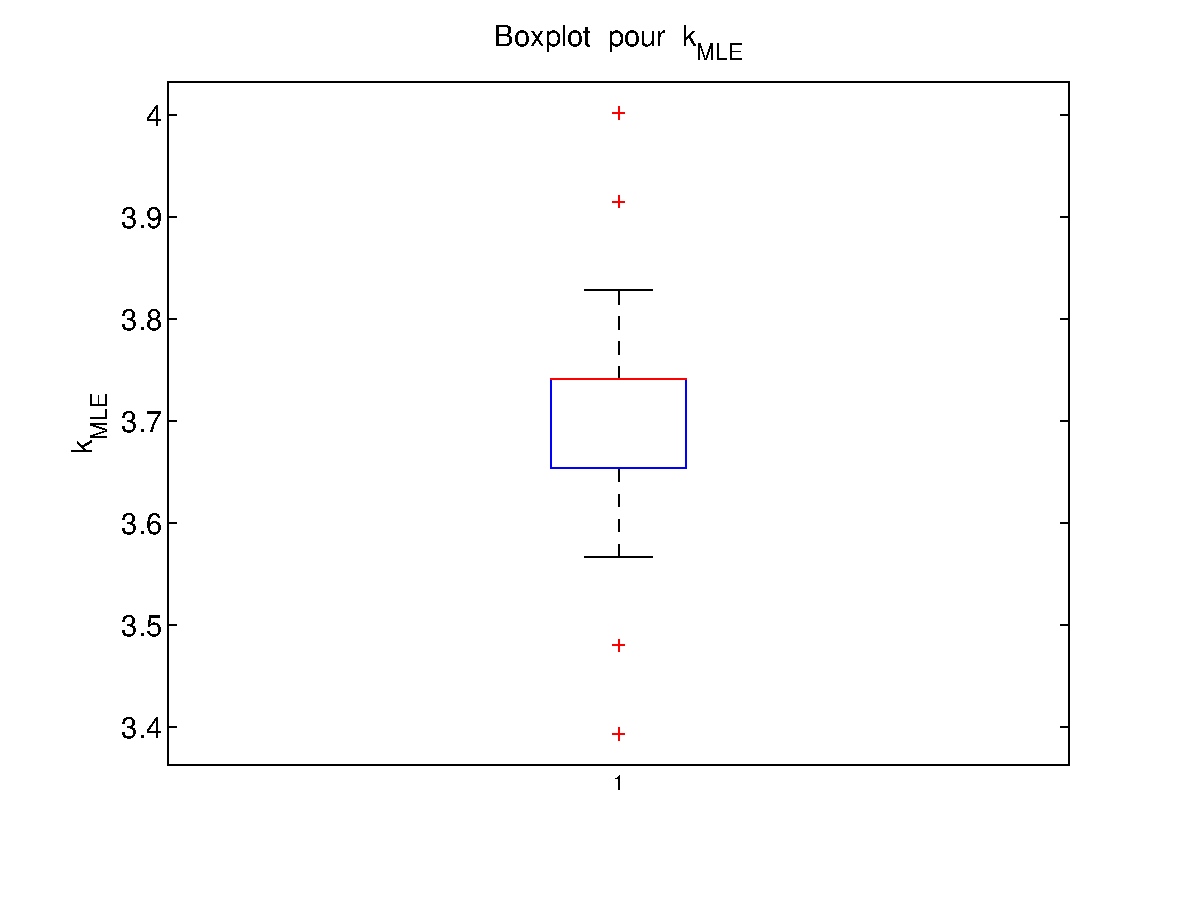
\includegraphics[width=\textwidth]{graphes/boxplot_kmle.eps}
        \end{subfigure}%
        ~
        \begin{subfigure}[b]{0.5\textwidth}
                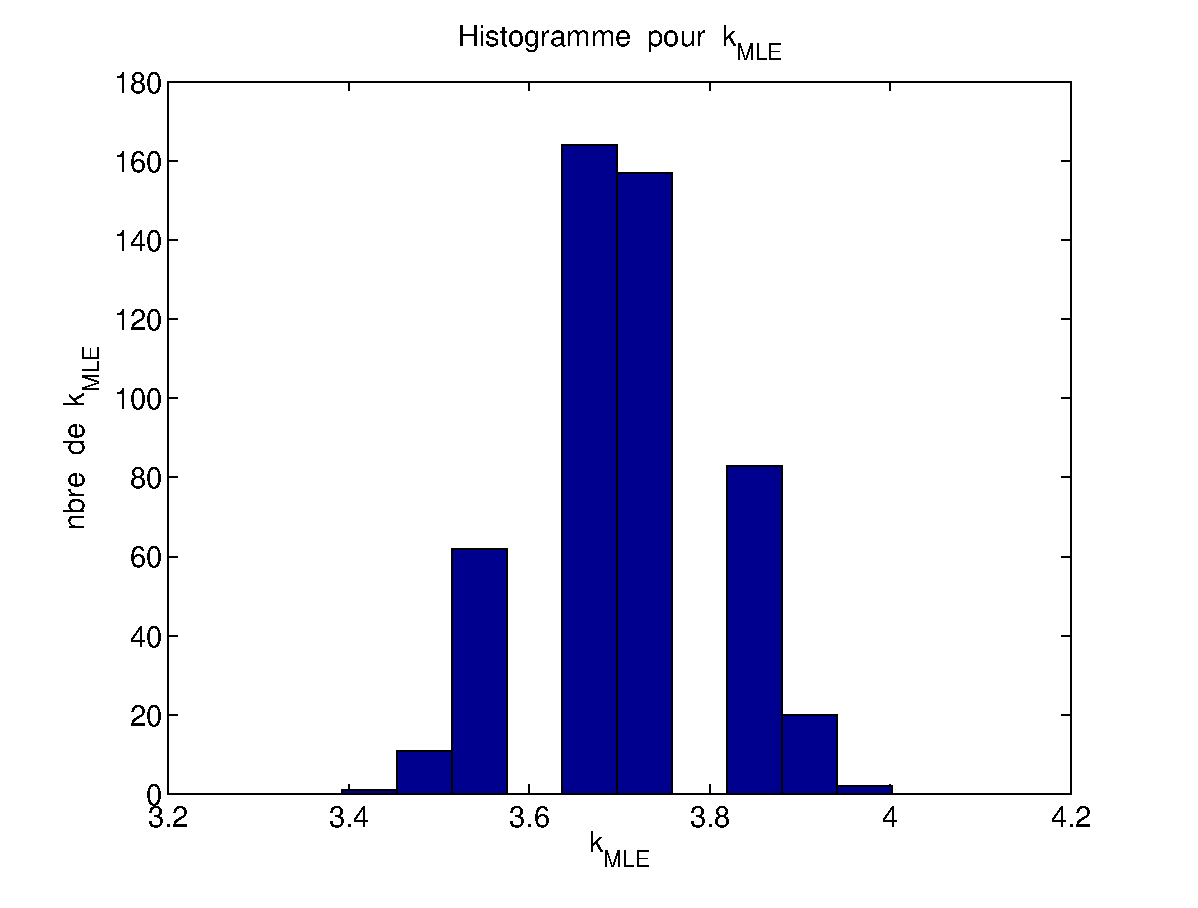
\includegraphics[width=\textwidth]{graphes/hist_kmle.eps}
        \end{subfigure}
        \caption{Graphes pour $\hat{k}_{MLE}$}\label{fig:kmle}
\end{figure}

\begin{figure}[!ht]
        \centering
        \begin{subfigure}[b]{0.5\textwidth}
                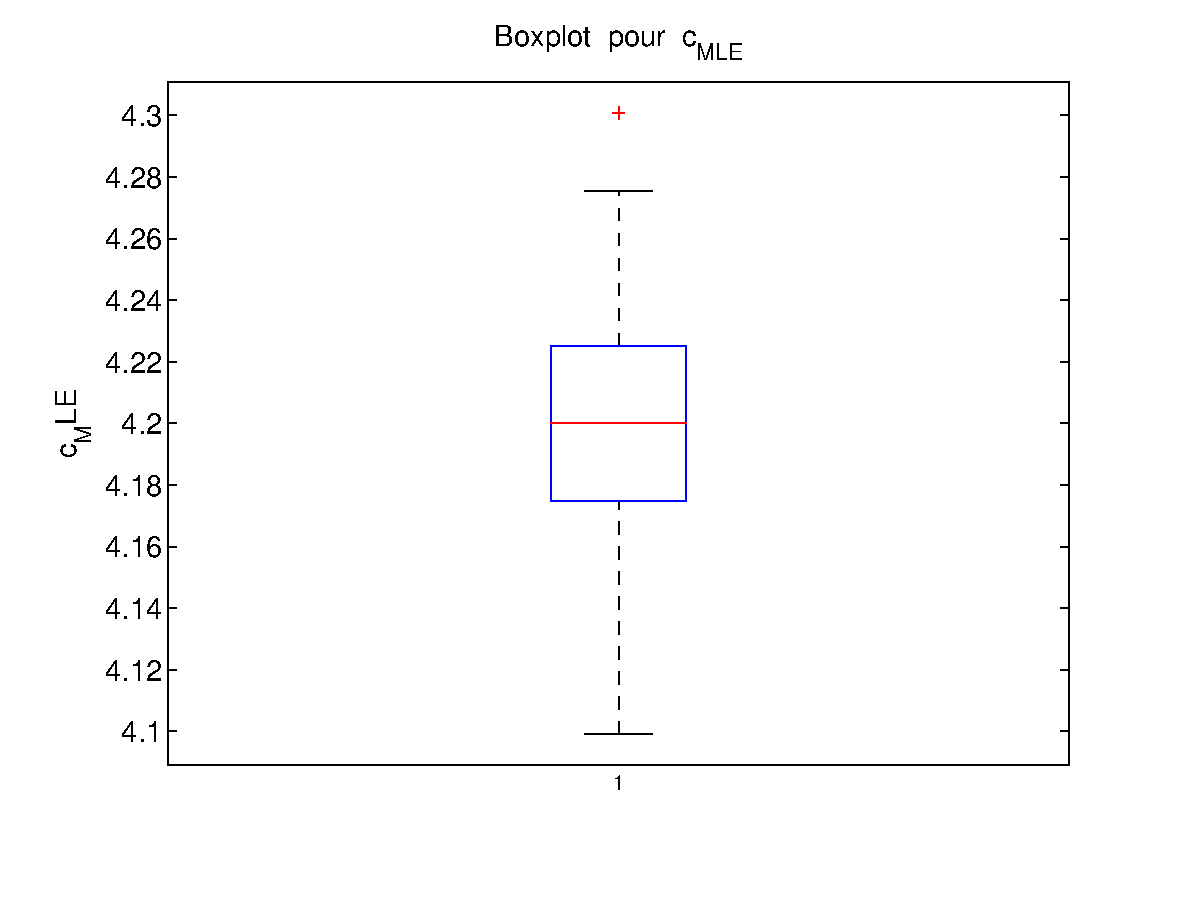
\includegraphics[width=\textwidth]{graphes/boxplot_cmle.eps}
        \end{subfigure}%
        ~
        \begin{subfigure}[b]{0.5\textwidth}
                \includegraphics[width=\textwidth]{graphes/hist_cmle.eps}
        \end{subfigure}
        \caption{Graphes pour $\hat{c}_{MLE}$}\label{fig:cmle}
\end{figure}

\begin{figure}[!ht]
        \centering
        \begin{subfigure}[b]{0.5\textwidth}
                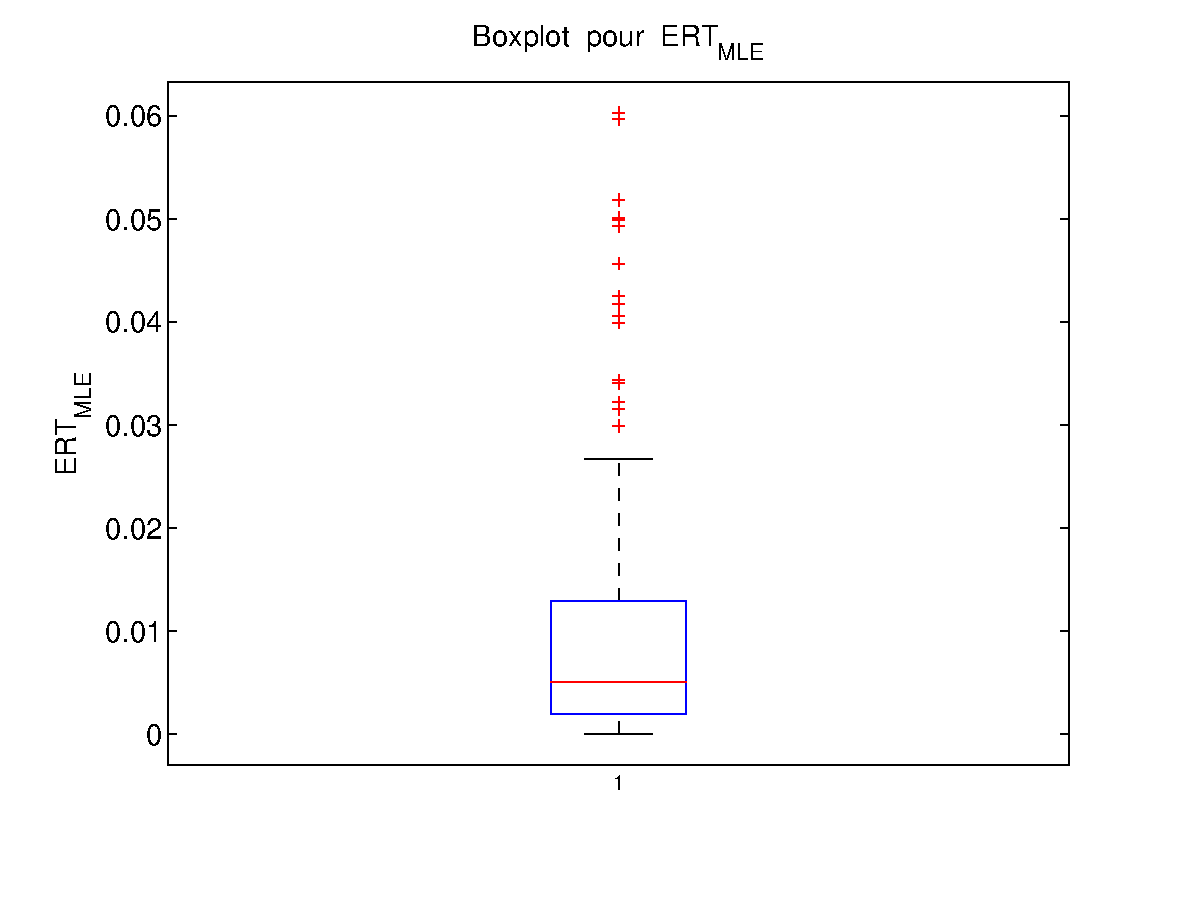
\includegraphics[width=\textwidth]{graphes/boxplot_ertmle.eps}
        \end{subfigure}%
        ~ 
        \begin{subfigure}[b]{0.5\textwidth}
                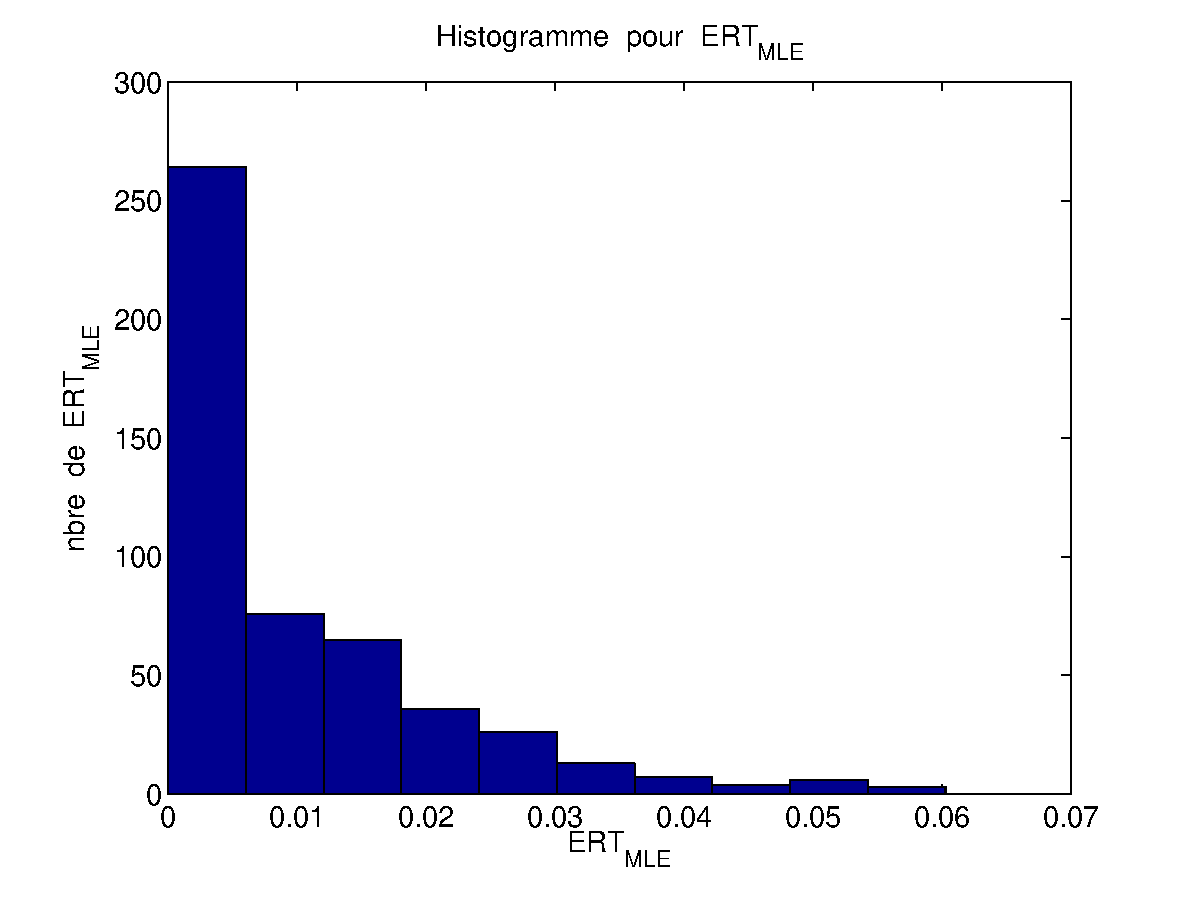
\includegraphics[width=\textwidth]{graphes/hist_ertmle.eps}
        \end{subfigure}
        \caption{Graphes pour $ERT_{MLE}$}\label{fig:ertmle}
\end{figure}

\paragraph{Biais, variance, consistence et distribution asymptotique}
La biais de notre estimateur $\hat{\theta}_{MLE}$ est négligeable; on peut donc raisonnablement dire qu'il est approximativement non-biaisé. En prenant des échantillons de plus en plus grand, on observe que la variance ne change pas significativement. $\hat{\theta}_{MLE}$ est donc non consistant.
En ce qui concerne les distributions asymptotiques, les histogrammes montrent qu'elles sont approximativement normales. Notons toutefois que ces propriétés dépendent grandement des intervalles et du nombre de  points candidats choisis initialement~: avec un intervalle plus grand autour des valeur réelles de $c$ et $k$, ou avec moins de points candidats, les résultats auraient été moins proches.



\subsection{Comparaison}
Comparons les trois méthodes utilisées pour $n = 500$. Nous prendrons en compte l'erreur quadratique totale et la variance des estimateurs et de l'erreur. Le tableau des valeurs est repris à la table~\ref{table:comp}.
Nous pouvons voir que la méthode graphique minimise l'erreur quadratique moyenne. C'est également cette méthode qui donne les variance de $\hat{k}$, $\hat{c}$ et $ERT$ les plus petites, ce qui signifie que les valeurs successives obtenues ont un écart moindre par rapport à la moyenne.

\begin{table}[!h]
\centering
\begin{tabular}{|l|l|l|}
\hline
				& Moyenne	& Variance\\
\hline
$\hat{k}_{MM}$	&			& 0.0085\\
$\hat{k}_{MG}$	&			& 0.0044\\
$\hat{k}_{MLE}$	&			& 0.0086\\
\hline
$\hat{c}_{MM}$	&			& 0.0014\\
$\hat{c}_{MG}$	&			& 0.0012\\
$\hat{c}_{MLE}$	&			& 0.0014\\
\hline
$ERT_{MM}$		& 0.0098	& 0.0001\\
$ERT_{MG}$		& 0.0057	& $4.0814\cdot 10^{-5}$\\
$ERT_{MLE}$		& 0.0100	& 0.0001\\
\hline
\end{tabular}
\caption{Comparaison des 3 méthodes d'estimation, $n = 500$}
\label{table:comp}
\end{table}

\section{Question 2}
\begin{enumerate}
  \item
    \begin{mytable}{val}{Table de différentes valeures des notes du test.}
      \begin{tabular}{ll}
        $n$                      & \np{252}\\
Moyenne                  & \np{1.059524e+01}\\
M\'ediane                & \np{1.050000e+01}\\
\'Ecart-type             & \np{2.642711e+00}\\
\'Etendue                & \np{1.250000e+01}\\
Coefficient de variation & \np{2.494244e-01}\\
Proportion de r\'eussite & \np{3.452381e-01}\\

      \end{tabular}
    \end{mytable}
  \item Utilisons la méthode des moments
    (qui donne la même chose que celle du maximum de vraissemblance pour
    une loi normale de toute façon).
    \begin{itemize}
      \item
        Pour la loi normale, on a
        \begin{align*}
          \bar{y} & = E(Y)\\
                  & = \mu\\
          \bar{y^2} & = E(Y^2)\\
                    & = \var(Y) + E(Y)^2\\
                    & = \sigma^2 + \mu^2
        \end{align*}
        ce qui donne
        \begin{align*}
          \mu & = \bar{y}\\
          \sigma^2 & = \bar{y^2} - \bar{y}^2.
        \end{align*}
      \item
        Pour la loi de Weibull, on a
        \begin{align*}
          \bar{y} & = E(Y)\\
                  & = \sqrt[m]{\alpha}\Gamma\left(1 + \frac{1}{m}\right)\\
          \bar{y^2} & = E(Y^2)\\
                    & = \var(Y) + E(Y)^2\\
                    & = \alpha^{2/m}\left(\Gamma\left(1 + \frac{2}{m}\right) -
                    \Gamma^2\left(1 + \frac{1}{m}\right)\right) + \alpha^{2/m}\Gamma^2\left(1 + \frac{1}{m}\right)\\
                    & = \alpha^{2/m}\Gamma\left(1 + \frac{2}{m}\right)
        \end{align*}
        ce qui donne
        \begin{align*}
          \mu & = \bar{y}\\
          \sigma^2 & = \bar{y^2} - \bar{y}^2.
        \end{align*}
    \end{itemize}
  \item
    La figure~\ref{fig:distrib} donne quelques exemple de distribution normale et de Weibull.
    On remarque que la distribution de Weibull a $f(x; \alpha, m) = 0$ $\forall x \leq 0$
    ce qui a du sens dans ce cas car une note ne peut pas être négative alors que
    la distribution normale a $f(x) > 0$ pour $f \leq 0$ même si la valeur est très faible
    si $\mu > 0$ et que $\sigma^2$ est suffisamment petit.

    \begin{figure}
      \centering
      \begin{subfigure}[b]{0.45\textwidth}
        \includegraphics[width=\textwidth]{img/normal.png}
        \caption{Normal distribution}
        \label{fig:normal}
      \end{subfigure}%
      ~ %add desired spacing between images, e. g. ~, \quad, \qquad etc.
      %(or a blank line to force the subfigure onto a new line)
      \begin{subfigure}[b]{0.45\textwidth}
        \includegraphics[width=\textwidth]{img/weibull}
        \caption{Weibull distribution}
        \label{fig:weibull}
      \end{subfigure}
      \caption{Comparison for Weibull and Normal distributions}
      \label{fig:distrib}
    \end{figure}
    De plus, la distribution normale est symétrique autour de $\mu$ alors que la distribution
    des notes d'un test n'est pas spécialement symétrique.
\end{enumerate}

\appendix

\section{Codes}
\matlabcode{val}{Cette fonction calculer différentes valeurs statistiques
des notes du test.}


\end{document}

